\documentclass[11pt,landscape,a4paper]{article}
\usepackage[utf8]{inputenc}
\usepackage[ngerman]{babel}
\usepackage[T1]{fontenc}
%\usepackage[LY1,T1]{fontenc}
%\usepackage{frutigernext}
%\usepackage[lf,minionint]{MinionPro}
\usepackage{tikz}
\usetikzlibrary{shapes,positioning,arrows,fit,calc,graphs,graphs.standard}
\usepackage[nosf]{kpfonts}
\usepackage[t1]{sourcesanspro}
\usepackage{multicol}
\usepackage{wrapfig}
\usepackage[top=4mm,bottom=4mm,left=4mm,right=4mm]{geometry}
\usepackage[framemethod=tikz]{mdframed}
\usepackage{microtype}
\usepackage{pdfpages}
\usepackage[shortlabels]{enumitem}

\newif\iflong
\longtrue % \longfalse for short version and \longtrue for long version
\newcommand{\inLongVersion}[1]{\iflong #1\fi}


\setlist{nosep}
\setlist[itemize]{leftmargin=*}
\setlist[enumerate]{leftmargin=*}

\newcommand{\score}{\text{score}}
\newcommand{\encoder}{\text{encoder}}
\newcommand{\decoder}{\text{decoder}}
\newcommand{\E}{\mathbb{E}}
\newcommand{\Dist}{\mathcal{D}}
\newcommand{\normal}{\mathcal{N}}
\DeclareMathOperator{\cov}{\textbf{Cov}}
\DeclareMathOperator{\var}{\textbf{Var}}
\DeclareMathOperator{\argmin}{\textbf{argmin}}
\DeclareMathOperator{\argmax}{\textbf{argmax}}
\DeclareMathOperator{\sgn}{\textbf{sgn}}
\DeclareMathOperator{\dir}{\textbf{Dir}}
\DeclareMathOperator{\cat}{\textbf{Cat}}






\let\bar\overline

\definecolor{myblue}{cmyk}{0,0,0,1}


\def\firstcircle{(0,0) circle (1.5cm)}
\def\secondcircle{(0:2cm) circle (1.5cm)}

\colorlet{circle edge}{myblue}
\colorlet{circle area}{myblue!5}

\tikzset{filled/.style={fill=circle area, draw=circle edge, thick},
    outline/.style={draw=circle edge, thick}}
    
\pgfdeclarelayer{background}
\pgfsetlayers{background,main}

\everymath\expandafter{\the\everymath \color{myblue}}
\everydisplay\expandafter{\the\everydisplay \color{myblue}}

\renewcommand{\baselinestretch}{.8}
\pagestyle{empty}

\global\mdfdefinestyle{header}{%
linecolor=gray,linewidth=1pt,%
leftmargin=0mm,rightmargin=0mm,skipbelow=0mm,skipabove=0mm,
}

\newcommand{\header}{
\begin{mdframed}[style=header]
\footnotesize
\sffamily
\centering
AML, Yuhao Mao,~Page~\thepage
\end{mdframed}
}

\makeatletter % Author: https://tex.stackexchange.com/questions/218587/how-to-set-one-header-for-each-page-using-multicols
\renewcommand{\section}{\@startsection{section}{1}{0mm}%
                                {.5ex}%
                                {.5ex}%x
                                {\color{myblue}\sffamily\bfseries}}
\renewcommand{\subsection}{\@startsection{subsection}{2}{0mm}%
                                {.2ex}%
                                {.2ex}%x
                                {\sffamily\bfseries}}
\renewcommand{\subsubsection}{\@startsection{subsubsection}{3}{0mm}%
                                {.1ex}%
                                {.1ex}%x
                                {\sffamily\itshape}}



\def\multi@column@out{%
   \ifnum\outputpenalty <-\@M
   \speci@ls \else
   \ifvoid\colbreak@box\else
     \mult@info\@ne{Re-adding forced
               break(s) for splitting}%
     \setbox\@cclv\vbox{%
        \unvbox\colbreak@box
        \penalty-\@Mv\unvbox\@cclv}%
   \fi
   \splittopskip\topskip
   \splitmaxdepth\maxdepth
   \dimen@\@colroom
   \divide\skip\footins\col@number
   \ifvoid\footins \else
      \leave@mult@footins
   \fi
   \let\ifshr@kingsaved\ifshr@king
   \ifvbox \@kludgeins
     \advance \dimen@ -\ht\@kludgeins
     \ifdim \wd\@kludgeins>\z@
        \shr@nkingtrue
     \fi
   \fi
   \process@cols\mult@gfirstbox{%
%%%%% START CHANGE
\ifnum\count@=\numexpr\mult@rightbox+2\relax
          \setbox\count@\vsplit\@cclv to \dimexpr \dimen@-1cm\relax
\setbox\count@\vbox to \dimen@{\vbox to 1cm{\header}\unvbox\count@\vss}%
\else
      \setbox\count@\vsplit\@cclv to \dimen@
\fi
%%%%% END CHANGE
            \set@keptmarks
            \setbox\count@
                 \vbox to\dimen@
                  {\unvbox\count@
                   \remove@discardable@items
                   \ifshr@nking\vfill\fi}%
           }%
   \setbox\mult@rightbox
       \vsplit\@cclv to\dimen@
   \set@keptmarks
   \setbox\mult@rightbox\vbox to\dimen@
          {\unvbox\mult@rightbox
           \remove@discardable@items
           \ifshr@nking\vfill\fi}%
   \let\ifshr@king\ifshr@kingsaved
   \ifvoid\@cclv \else
       \unvbox\@cclv
       \ifnum\outputpenalty=\@M
       \else
          \penalty\outputpenalty
       \fi
       \ifvoid\footins\else
         \PackageWarning{multicol}%
          {I moved some lines to
           the next page.\MessageBreak
           Footnotes on page
           \thepage\space might be wrong}%
       \fi
       \ifnum \c@tracingmulticols>\thr@@
                    \hrule\allowbreak \fi
   \fi
   \ifx\@empty\kept@firstmark
      \let\firstmark\kept@topmark
      \let\botmark\kept@topmark
   \else
      \let\firstmark\kept@firstmark
      \let\botmark\kept@botmark
   \fi
   \let\topmark\kept@topmark
   \mult@info\tw@
        {Use kept top mark:\MessageBreak
          \meaning\kept@topmark
         \MessageBreak
         Use kept first mark:\MessageBreak
          \meaning\kept@firstmark
        \MessageBreak
         Use kept bot mark:\MessageBreak
          \meaning\kept@botmark
        \MessageBreak
         Produce first mark:\MessageBreak
          \meaning\firstmark
        \MessageBreak
        Produce bot mark:\MessageBreak
          \meaning\botmark
         \@gobbletwo}%
   \setbox\@cclv\vbox{\unvbox\partial@page
                      \page@sofar}%
   \@makecol\@outputpage
     \global\let\kept@topmark\botmark
     \global\let\kept@firstmark\@empty
     \global\let\kept@botmark\@empty
     \mult@info\tw@
        {(Re)Init top mark:\MessageBreak
         \meaning\kept@topmark
         \@gobbletwo}%
   \global\@colroom\@colht
   \global \@mparbottom \z@
   \process@deferreds
   \@whilesw\if@fcolmade\fi{\@outputpage
      \global\@colroom\@colht
      \process@deferreds}%
   \mult@info\@ne
     {Colroom:\MessageBreak
      \the\@colht\space
              after float space removed
              = \the\@colroom \@gobble}%
    \set@mult@vsize \global
  \fi}

\makeatother
\setlength{\parindent}{0pt}




\begin{document}
%\footnotesize
\small
\begin{multicols*}{4}

    \section{Maximum Likelihood Estimator}
\begin{itemize}[itemsep=0pt,topsep=0pt, leftmargin=2pt, itemindent=5pt, labelwidth=5pt]
    \item Consitent,asymptotic unbiased.$\hat{\theta}^{\mathrm{MLE}}_n\overset{\mathbb{P}}{\to}\theta_0$.
    \item Asymptotic normal. $\sqrt{n}(\hat{\theta}^{\mathrm{MLE}}_n-\theta_0) \overset{\mathcal{D}}{\to} \normal(0, I_n)$, $I_n(\theta_0)= \mathbb{E}[- \dot{s}_\theta ] = \mathbb{E}[s_\theta s_\theta^{\top}]$ fisher info, $s_\theta(x) = \partial_\theta \ln p_\theta(x)$ score func, $\mathbb{E}_{\theta}s_\theta = 0$.
    \item Asymptotic efficient. $\hat{\theta}^{\mathrm{MLE}}_n$ reaches CRLB when $n\rightarrow \infty$. $\hat{\theta}^{\mathrm{MLE}}$ not  efficient if $n$ finite. Stein estimator always better.
    \item Equivariance, if $\hat{\theta}_n$ is MLE, $\hat{\gamma} = g(\hat{\theta}^{\mathrm{MLE}})$ is MLE of $\mathcal{L}(g^{-1}(\gamma))$. Proof by optimally of MLE.
\end{itemize}

Cramer-Rao lower bound (CRLB): for any \emph{unbiased} $\hat{\theta}$ of $\theta_0$, $\E (\hat{\theta}-\theta_0)^2 \ge 1/I_n(\theta_0)$

Proof: $\text{Cov}[s_\theta, \hat{\theta}] = \mathbb{E}[s_\theta \cdot \hat{\theta}] = \partial_\theta  \mathbb{E}[\hat{\theta}] = \partial_\theta \theta = 1$. Cauchy-Schwarz $\text{Cov}^2[s_\theta, \hat{\theta}]\leq \text{Var}[s_\theta] \text{Var}[\hat{\theta}] = I_n(\theta) \E (\hat{\theta}-\theta_0)^2$ QED.
% define $\Lambda = \frac{\partial \log P(X;\theta)}{\partial \theta}$. Cauchy-Schwarz says $\cov^2(\Lambda, \hat{\theta})\le \var(\Lambda)\var(\hat{\theta}) = \E(\Lambda^2) \var(\hat{\theta})$ because $\E \Lambda=0$. Note that $\cov(\Lambda, \hat{\theta}) = \E(\Lambda\hat{\theta}) = \int_X \hat{\theta}(x) \frac{\partial}{\partial \theta}f(x;\theta) dx = \frac{\partial}{\partial \theta} \int_X \hat{\theta}(x) f(x;\theta) dx = \frac{\partial}{\partial \theta} \E \hat{\theta} = 1$. Therefore, $\var(\hat{\theta}) \ge 1/\E(\Lambda^2)$.

However, when dimension of problem goes to infinity while data-dim ratio is fixed, MLE is biased and the $p$-values are unreliable. 


    \section{Regression}

\subsection*{Bias-Variance trade-off}
$\mathcal{D}$ training dataset, $\hat{f}$ predictive function.
$ \E_D \E_{Y\mid X} (\hat{f}(X)-Y)^2 = \E_D (\hat{f}(x)-\E_D \hat{f}(x))^2 + \left(\E_D \hat{f}(x)-\E(Y\mid X)\right)^2 + \E_D (\E(Y\mid X)-Y)^2 = \text{Model Variance} + \text{Bias}^2 + \text{Intrinsic Noise}$. 

The optimal trade-off is achieved by avoiding under-fitting (large bias) and over-fitting (large variance). Note that here the variance of output is computed by refitting the regressor on a new dataset.

\subsection*{Regularization}

Ridge and Lasso can be viewed as MAP estimation with a prior on $\beta$. Ridge = Gaussian Prior and LASSO = Laplacian prior. Using SVD, we get Ridge has built-in model selection:  $X\beta^{\text{Ridge}} = \sum_{j=1}^d [d_j^2 /(d_j^2+\lambda)] u_j u_j^T Y$ (each $u_j u_j^T Y$ can be viewed as a model). Lasso has more sparse estimations because the gradient of regularization does not shrink as Ridge.


    \section{BLR and GP}

\subsection*{Bayesian Linear Regression}
Model $Y=X\beta+\epsilon$, $\epsilon\sim \normal(0, \sigma^2)$. Prior $\beta \sim \normal(0, \Lambda^{-1})$. Posterior $\beta \mid X, Y \sim \normal(\mu_\beta, \Sigma_\beta)$, where $\mu_\beta = (X^T X+\sigma^2\Lambda)^{-1}X^T Y$ and $\Sigma_\beta =  (\sigma^{-2}X^T X+\Lambda)^{-1}$.  

% MAP estimation of this prior (i.e., $\mu_\beta$) is equivalent to Ridge regression given $\Lambda = \lambda I$ and $\sigma=1$.

% When $\Lambda=\lambda I$, under the prior, $Y\sim \normal(0, \frac{1}{\lambda}X^T X+\sigma^2 I)$. Therefore, $\cov(y_i, y_j) = \frac{1}{\lambda}x_i^T x_j$. It means a prior that closer samples is more similar, i.e., $\cov(y_i, y_j)$ is large when $x_i^T x_j$ is large. The kernel $X^T \Lambda^{-1} X$ is thus called linear kernel. When a general kernel is used, Gaussian Process appears.

\subsection*{Gaussian Process}
$Y = \left(\begin{matrix} Y_0 \\ Y_1 \end{matrix}\right)$ is the combination of observed and prediction value. Assume a Gaussian prior of $\mathcal{N}(0, K + \sigma^2 I)$, where $K_{ij}=k(x_i,x_j)$ is kernel. GP regression is the conditional/Posterior distribution on $Y_0$, $\mathbb{E} [Y_1|Y_0] = K_{1 0}(\sigma^{2} I_{0}+K_{00})^{-1}Y_0$, $\mathrm{Cov}[Y_1] = \sigma^{2}I_{1} + K_{11} - K_{10} (\sigma^2  I_{0} + K_{00})^{-1} K_{01}$. Bayesian LR is a special case of GP with linear kernel $k(x,y) = x^{\top}\Lambda^{-1}y$.

\subsection*{Kernel Function}
A function is a kernel iff (1) symmetry $k(x, x^\prime)=k(x^\prime, x)$ and (2) semi-positive definite $\int_\Omega k(x, x^\prime) f(x) f(x^\prime) dx dx^\prime \ge 0$ for any $f \in L_2$ and $\Omega \in \mathcal{R}^d$ (continuous) or $K(X)\succeq 0$ (discrete). The latter is equivalent to (1) $a^{\top} K a \geq 0, \forall a$ or (2) $k(x, x^\prime) = \phi(x)^T \phi(x^\prime)$ for some $\phi$.

\subsection*{Kernel Construction}
If $k_{1,2}$ are valid kernels, then followings are valid: (1) $k(x, x^\prime) = k_1(x, x^\prime) + k_2(x, x^\prime)$. (2) $k(x, x^\prime) = k_1(x, x^\prime)\cdot k_2(x, x^\prime)$. Proof: let $V\sim \normal(0, K_1)$, $W\sim \normal(0, k_2)$ and is independent to $V$, then $\cov(V_i W_i, V_j W_j) = \cov(V_i, V_j)\cov(W_i, W_j) = k_1\cdot k_2(x_i, x_j)$. (3) $k(x, x^\prime) = c k_1(x, x^\prime)$ for constant $c>0$. (4) $k(x, x^\prime) = f(k_1(x, x^\prime))$ if $f$ is a polynomial with positive coefficients or the exp. Proof: polynomial can be proved by applying the product, positive scaling and addition. Exp can be proved by taking limit on the polynomial. (5) $k(x, x^\prime) = f(x) k_1(x, x^\prime) f(x^\prime)$. (6) $k(x, x^\prime) = k_1(\phi(x), \phi(x^\prime))$ for any function $\phi$.


Example: RBF kernel $k(x,y) = \exp(-||x-y||^2/2\sigma^2) = \exp(-||x||^2/2\sigma^2) \times \exp(x^T y/2\sigma^2) \times \exp(-||y||^2/2\sigma^2)$ is valid. (1) $x^T y$ linear kernel is valid (2) then $\exp(\frac{1}{\sigma^2}x^T y)$ is valid, (3) let $f(x) = \exp(-\frac{1}{2\sigma^2} ||x||^2)$, by rules $f(x) k(x, y) f(y)$ RBF is valid.

\textbf{Mercer's Theorem}: Assume $k(x, x^\prime)$ is a valid kernel. Then there exists an orthogonal basis $e_i$ and $\lambda_i\ge 0$, s.t. $k(x, x^\prime) = \sum_{i} \lambda_i e_i(x) e_i(x^\prime)$.




    \section{Linear Methods for Classification}

\subsection*{Concept Comparison}

\begin{enumerate}
    \item Probabilistic Generative, modeling $p(x, y)$: (1) can create new samples, (2) outlier detection, (3) probability for prediction, (4) high computational cost and (5) high bias.
    \item Probabilistic Discriminative, modeling $p(y\mid x)$: (1) probability for prediction, (2) medium computational cost and (3) medium bias.
    \item Discriminative, modeling $y=f(x)$: (1) no probability for prediction, (2) low computational cost and (3) low bias.
\end{enumerate}

\subsection*{Infer $p(x,y)$ for classification problems}

Use $p(x,y) = p(y)p(x\mid y)$. Since $y$ has finite states, model $p(y)$ and $p(x\mid y)$ for different $y$. The modeling requires to (1) guess a distribution family and (2) infer parameters by MLE.

\subsection*{Compute $p(y\mid x)$ by discriminant analysis (DA)}

\subsubsection*{Linear DA}

Goal: classify a sample into two Gaussian distribution with $\Sigma_0 = \Sigma_1$.
After calculation, $p(y=1\mid x) = 1/(1+\exp(-\log\frac{p(x\mid y=1)p(y=1)}{p(x\mid y=0)p(y=0)})) = 1/(1+\exp(w_1^T x +w_0))$ since the quadratic term is eliminated due to $\Sigma_0=\Sigma_1$.

\subsubsection*{Quadratic DA}

Goal: classify a sample into two Gaussian distribution with $\Sigma_0 \ne \Sigma_1$.
After calculation, $p(y=1\mid x) = 1/(1+\exp(x^T W x + w_1^T x +w_0))$.

\subsection*{Optimization Methods}

\subsubsection*{Optimal Learning Rate for Gradient Descent}

Goal: find $\eta^* = \argmin_\eta L(w^k - \eta\cdot \nabla L(w^k))$. By Taylor expansion of $L(w^{k+1})$ at $w^k$ and solve for the optimal $\eta$, we get $\eta^* = \frac{||\nabla L(w^k)||^2}{\nabla L(w^k)^T H_L(w^k) \nabla L(w^k)}$.

However, naive gradient descent has two weaknesses: (1) it often has a zig-zag behavior, especially in a very narrow, long and slightly downward valley; (2) the gradient update is small near the stationary point. This can be mitigated by adding a momentum term in the update: $w^{k+1} = w^k -\eta \nabla L(w^k) + \mu^k (w^k -w^{k-1})$ which speeds the update towards the ``common'' direction.

\subsubsection*{Newton's Method}

Taylor-expand $L(w)$ at $w_k$ to derive the optimal $w^{k+1}$: $L(w) \approx L(w) + (w-w^k)^T \nabla L(w^k) + \frac{1}{2}(w-w^k)^T H_L(w^k) (w-w^k) \Rightarrow w^{k+1} = w^k - H_L^{-1}(w^k)\nabla L(w^k)$. 

Pros: (1) better updates compared to GD since it uses the second Taylor term and (2) does not require learning rate.

Cons: requires $H_L^{-1}$ which is expensive.

\subsection*{Bayesian Method}

In most cases, the posterior is intractable. Use approximation of posterior instead.

\subsubsection*{Laplacian Method}

Idea: approximate posterior near the MAP estimation with a Gaussian distribution.
$p(w\mid X, Y) \propto p(w, X, Y) \propto \exp(-R(w))$, where $R(w) = -\log p(w, X, Y)$. Let $w^* = \argmin R(w)$ be the MAP estimation and Taylor-expand $R(w)$ at $w^*$: $R(w) \approx R(w^*) + \frac{1}{2}(w-w^*)^T H_R(w^*) (w-w^*)$. Therefore, $p(w\mid X,Y)\propto \exp(-R(w^*) -\frac{1}{2}(w-w^*)^T H_R(w^*) (w-w^*))$ and thus $(w\mid X,Y) \sim \normal(w^*, H_R^{-1}(w^*))$.

\subsubsection*{AIC \& BIC}

% We use prior $w\sim \normal(\mu_0, \alpha_0 I_d)$ for $\alpha_0$ sufficiently large (little prior). Since $p(w\mid X, Y) = p(w, X, Y) / p(X, Y) \approx \exp(-R(w^*) -\frac{1}{2}(w-w^*)^T H_R(w^*) (w-w^*)) / p(X, Y)$ is a Gaussian distribution, we have $p(X, Y)\approx e^{-R(w^*)}(2\pi)^{-d/2}|H_R(w^*)|^{-1/2}$. Therefore, $\log p(X,Y)\approx -R(w^*) -\frac{d}{2}\log(2\pi) - \frac{1}{2}\log |H_R(w^*)| = \log p(w^*) + \log p(X, Y\mid w^*)-\frac{d}{2}\log(2\pi) - \frac{1}{2}\log |H_R(w^*)|$. Further, notice that $H_R(w^*) = \frac{\partial^2}{\partial ww^T}(-\log p(w^*)-\log p(X, Y \mid w^*)) = -(\alpha_0 I_d)^{-1} - N \E_{x, y} (\frac{\partial^2}{\partial ww^T} \log p(x,y\mid w^*)) \approx N \mathbf{I}$, where $\mathbf{I}$ is the fisher information.
\begin{itemize}
    \item Define BIC = $k\log N -2\log \hat{L}$, where $k$ is \#parameters and $\hat{L}$ is the likelihood $p(x\mid w^*)$. A lower BIC means a better model.
    \item Define AIC = $2k-2\log \hat{L}$. A lower AIC means a better model.
\end{itemize}

\subsection*{LDA by loss minimization}

\subsubsection*{Perceptron}

Goal: for $y_i\in\{0,1\}$, find $w$, s.t. $y_i w^T x_i >0$ for any $i$. The classification function is $c(x) = \sgn(w^T x)$.

$L(y, c(x)) = 0$ if $y w^T x >0$ and $L(y, c(x)) = -y w^T x$ o.w. By gradient descent, the Perceptron is guaranteed to converge if (1) the data is linearly separable, (2) learning rate $\eta(k)>0$, (3) $\sum_k \eta(k) \rightarrow +\infty$ and (4) $(\sum_k \eta(k)^2)/(\sum_k \eta(k))^2 \rightarrow 0$. However, there exists multiple solutions if the data is linearly separable.

\subsubsection*{Fisher's LDA}

Idea: project the two distribution into one dimension and maximize the ratio of the variance between the classes and the variance within the classes, i.e., $\max (w^T u_1-w^T u_0)^2/(w^T S w)$, where $S = \Sigma_0+\Sigma_1$. Let gradient be zero and solve for $w^*$, we get $w^*\propto S^{-1}(u_1-u_0)$.

We first compute $w^*$ and fit distributions of the two-class projection. Then apply Bayesian decision theory to make classification.


    \section{Convex Optimization}

Definition: the objective is convex and the feasible set is convex. The standard form is to minimize a convex function ($f(w)$ for convex $f$) under affine equality constraint ($g_i(w)=0$ for affine $g_i$) and convex non-positive constraint ($h_i(w)\le 0$ for convex $h_i$).

\subsection*{How to Solve}

(1) Define Lagrangian: $L(w, \lambda, \alpha) = f(w)+\sum_i \lambda_i g_i(w) + \sum_j \alpha_j h_j(w)$ and $\alpha_j\ge 0$.

(2) Check whether strong duality holds using Slater's condition (sufficient but not necessary): there is a strictly feasible point, i.e., $\exists w_0$, s.t. $g_i(w_0)=0$ and $h_i(w_0)<0$.

(3) Solve for $dL(w)=0$, $g_i(w)=0$,  $\alpha\ge 0$, $h_j(w)\le 0$ and $\alpha_j h_j(w) = 0$ (complementary slackness).

(4) Weak duality always holds and when Slater's condition holds it equals  $\min_w f(w)$: solve $\max_{\lambda, \alpha} \Theta(\lambda, \alpha)$ s.t. $\alpha\ge 0$, where $\Theta(\lambda, \alpha) = \min_w L(w, \lambda, \alpha)$. The optimal in the weak duality is a lower bound for $\min_w f(w)$ since $\Theta(\lambda, \alpha)\le \min_w f(w)$ for any $\lambda$ and $\alpha$.

    \section{Support Vector Machine}
\subsection*{Linear Separable Case}
\textbf{Primal}: $\max_{w,b} \left\{\frac{1}{||w||} \min_{i}  y_{i}(w^{\top}x_{i}+b)\right\} \Leftrightarrow$

$\max_{w,b,t} t$ s.t. $\forall i,t\leq y_{i}(w^{\top}x_{i}+b)$ and $||w|| = 1$

$\Leftrightarrow \min_{w,b} \frac{1}{2} w^2$ s.t. $\forall i,1 \leq y_{i}(w^{\top}x_{i}+b)$ 

(1) KKT cond: $\forall i, \alpha_i \geq 0, (1-y_{i}(w^{\top}x_{i}+b))\leq 0, \alpha_{i}(1-y_{i}(w^{\top}x_{i}+b)) = 0$

(2) \textbf{Dual}: $\max_{\alpha} \sum_{i} \alpha_{i} - \frac{1}{2}\sum_{i,j}\alpha_{i} \alpha_{j} y_{i} y_{j} K(x_{i},x_{j})$ s.t. $(\alpha_i \geq 0)\land (\sum_{i} \alpha_{i} y_{i} = 0)$

\subsection*{Non-separable Case}
Introduce slack variables $\xi_i := \max \{1 - y_i(w^{\top}x_i + b), 0\} = [1 - y_i(w^{\top}x_i + b)]_{+}$ into loss. 

\textbf{Primal}: $\min_{w,b} \frac{1}{2} w^2 + C\sum_i\xi_i = \min_{w,b} \frac{1}{2} w^2 + C[1 - y_i(w^{\top}x_i + b)]_{+}$.  Hinge loss $[1-x]_{+}$.

Equivalent form: $\min_{w,b} \frac{1}{2} w^2 + C\sum_i\xi_i$ s.t. $ y_i(w^{\top}x_i + b) \geq 1-\xi_i$ and $\xi_i \geq 0$

\textbf{Dual}: $\max_{\alpha} \sum_{i} \alpha_{i} - \frac{1}{2}\sum_{i,j}\alpha_{i} \alpha_{j} y_{i} y_{j} K(x_i, x_j)$ s.t. $\sum_i \alpha_i y_i=0 $ and $0\leq \alpha_i \leq C$


\subsection*{Multi-class SVM}
$\min_{w=[w_{0:K-1}],b=[b_{0:K-1}]} \frac{1}{2} ||w||^2 + \sum_i C\xi_i$ s.t. $\xi_i\geq 0$ and $(w_{y_i}^{\top} x +b_{y_i}) - (w_{y}^{\top}x + b_{y}) \geq 1 -\xi_i, \forall y\neq y_i$

\subsection*{Structural SVM}
$y$ is structured, e.g. trees, maximum margin between $y_i,y_j$ depends on their similarity, so the condition changes to $w^{\top}\Psi(x_i,y_i)) - w^{\top}\Psi(x_i,y)) \geq \Delta(y_i,y) -\xi_i,\;\forall\;y\neq y_i$.
% \subsection*{Hard-Margin SVM}

% The optimization form is to minimize $\frac{1}{2}||w||^2$, s.t. $y_i(w^T x_i+w_0)\ge 1$ ($y_i\in \{-1,1\}$). It is convex and the Slater's condition holds under the assumption of linear separability.

% By solving $\min_{w, w_0} L(w, w_0, \alpha)$, the duality form is $\max_\alpha -\frac{1}{2}\sum_{i,j} \alpha_i \alpha_j y_i y_j x_i^T x_j+\sum_i \alpha_i$, s.t. $\alpha_i\ge 0$, $\sum_i \alpha_i y_i = 0$. $w^* = \sum_{i\in \text{support vec}} \alpha_i^* y_i x_i$.

% \subsection*{Soft-Margin SVM \& Kernel SVM}

% When the data is not linearly separable, one solution is to add slack variables: $\min_{\xi,w,w_0} \frac{1}{2}||w||^2+C\sum_i \xi_i$, s.t. $y_i(w^T x_i+w_0) \ge 1-\xi_i$ and $\xi_i\ge 0$. Note: when the data is linearly separable, soft-margin does not necessarily produce the same cut-plane as the hard-margin SVM, especially when the margin is small due to few support vectors. When $C\rightarrow\infty$, it becomes hard-margin SVM.

% The only difference in the dual form is that we need an extra condition $0\le \alpha\le C$. $\xi_i^* = \max(0, 1-y_i(w^{*T}x_i+w_0))$.

% Another solution, Kernel SVM, is to use $K(x_i, x_j) = \phi(x_i)^T \phi(x_j)$ to replace $x_i^T x_j$.

% \subsection*{Multi-class SVM}

% Idea: use M := \#class hyperplanes and maximize the generalized margin: $\min \sum_{i=1}^M w_i^T w_i$ s.t. $w_{y_i}^T x_i + w_{y_i, 0} - \max_{y\ne y_i} w_y^T x_i + w_{y,0} \ge 1$.

% \subsection*{Structural SVM}

% Goal: predict a structured output label, e.g., parsing trees.

% \inLongVersion{
% Difficulty of predicting structures:
% \begin{enumerate}
%     \item Compact representation of output space. Sol: use a score function and feature map $\hat{y}=\argmax_y w^T \Psi(x, y)$.
%     \item Efficient prediction (cannot use brute-force search to find argmax). Sol: assume structures such as decomposable output spaces.
%     \item Define prediction error (cannot use 0/1 errors). Sol: use a loss function $\Delta(y, \hat{y})$.
%     \item Efficient training (cannot evaluate all constraints). Sol: iteratively add new constraints to the training.
% \end{enumerate}
% }

% $\min _{\mathbf{w}, \boldsymbol{\xi} \geq 0} \frac{1}{2} \mathbf{w}^{\top} \mathbf{w}+C \sum_{i=1}^{n} \xi_{i}$, s.t. $\mathbf{w}^{\top} \Psi\left(z_{i}, \mathbf{y}_{i}\right)-\max _{z \neq z_{i}}\left[\Delta\left(z, z_{i}\right)+\mathbf{w}^{\top} \Psi\left(z, \mathbf{y}_{i}\right)\right] \geq-\xi_{i}, \forall \mathbf{y}_{i} \in \mathcal{Y}$.


    \section{Ensemble: Adaboost}

Adaboost has following properties:
\begin{enumerate}
    \item It minimizes exponential loss forwardly.
    \item It trains max-margin classifiers.
    \item It, as well as Random Forest, is spiky self-averaging interpolators, which localize the effect of noise.
    \item It falls into the double descent regime: over-parameterized models can have better generalization.
\end{enumerate}

    \section{Generative Models}

\textbf{ELBO} \begin{scriptsize}
    $\ln p(y) = \ln \int p(y \mid \theta) p(\theta) d \theta = \ln \mathbb{E}_{\theta \sim q}\left[p(y \mid \theta) \frac{p(\theta)}{q(\theta)}\right] \geq \mathbb{E}_{\theta \sim q}\left[\ln \left(p(y \mid \theta) \frac{p(\theta)}{q(\theta)}\right)\right]  = \mathbb{E}_{\theta \sim q}[\ln p(y \mid \theta)]-K L(q \| p(\cdot))$
\end{scriptsize}

\textbf{VAE} Goal: Find a latent representation $z$ of $x$ with simple prior $p_\theta(z)$. Problem: $p_\theta(x) = \mathbb{E}_{\theta}p(x|z)$ intractable. Solution: use encoder net $q_e(x|z)$ and $q_d(z|x)$ to model conditional and posterior prob.

\textbf{ELBO for VAE training} loss $l=\sum \ln \left(p_{\theta}\left(x_{i}\right)\right)$
\vspace{-0.4cm}
\begin{scriptsize}
    \begin{equation*}
        \begin{aligned}
             & \ln \left(p_{\theta}\left(x_{i}\right)\right)=\underset{Z \sim q_{\phi}\left(z \mid x_{i}\right)}{\mathbb{E}}\left[\ln p_{\theta}\left(x_{i}\right)\right] = \mathbb{E}_{Z}\left[\ln \frac{p_{\theta}\left(x_{i} \mid z\right) p_{\theta}(z)}{p_{\theta}\left(z \mid x_{i}\right)}\right]                               \\
             & = \mathbb{E}_{Z}\left[\ln \frac{p_{\theta}\left(x_{i} \mid z\right) p_{\theta}(z)}{p_{\theta}\left(z \mid x_{i}\right)} \frac{q_{\phi}\left(z \mid x_{i}\right)}{q_{\phi}\left(z \mid x_{i}\right)}\right]                                          \\
             & = \mathbb{E}_{Z}\left[\ln p_{\theta}\left(x_{i} \mid z\right)\right] - \mathbb{E}_{Z}\left[\ln \frac{q_{\phi}\left(z \mid x_{i}\right)}{p_{\theta}(z)}\right]+\mathbb{E}_{Z}\left[\ln \frac{q_{\phi}\left(z \mid x_{i}\right)}{p_{\theta}\left(z \mid x_{i}\right)}\right]                                                                                                                 \\
             & = \underbrace{\mathbb{E}_{Z}\left[\ln p_{\theta}\left(x_{i} \mid z\right)\right]-\mathrm{KL}\left(q_{\phi}\left(z \mid x_{i}\right) \| p_{\theta}(z)\right)}_{\text{ELBO }\mathcal{L}\left(x_{i}, \theta, \phi\right)} \\
             &+ \mathrm{KL}\left(q_{\phi}\left(z \mid x_{i}\right) \| p_{\theta}\left(z \mid x_{i}\right)\right) \geq \text{ELBO}.
        \end{aligned}
    \end{equation*}
\end{scriptsize}
\vspace{-0.4cm}

\textbf{Generative Adversarial Network}: Generator $G$ and Discriminator $D$. Optimize $\min _{G} \max _{D} V(D, G)$ where $V(D, G) = \mathbb{E}_{x \sim p_{\text {data }}(x)}[\ln D(x)]+\mathbb{E}_{z \sim p_{z}(z)}[\ln (1-D(G(z)))]$



\section{Convergence of SGD, Robbins-Monro}
Loss gradient $\ell(\cdot)$, SGD update $z^{(t)} \leftarrow \ell \theta^{(t)}+\gamma^{(t)}, \theta^{(t+1)} \leftarrow \theta^{(t)}-\eta(t) z^{(t)}$, $\gamma^{(t)}$ noise.

Problem: Whether $\theta^{\infty}\to \arg_{\theta^*}\mathbb{E}[\ell (\theta^*)]\triangleq 0$?

Assume: (1) $\mathbb{E}[\gamma] = 0$, (2) $\mathbb{E}[\gamma^2] = \sigma$ (3) $\left(\theta-\theta^{*}\right) \ell(\theta)>0,\forall \theta\neq\theta^*$ (4) $\exists b,\ell(\theta) < b,\forall \theta$. If (1) $\eta^{(t)}\to 0$ (2) $\underset{t<\infty}{\sum} \eta(t)=\infty$ (3) $\underset{t<\infty}{\sum} \eta^{2}(t)<\infty$, then $\mathbb{P}\left(\theta^{*}=\theta^{(t)}\right) \underset{t \rightarrow \infty}{\longrightarrow} 1$.

Proof:
\begin{scriptsize}
    $\mathbb{E}[(\theta^{(t+1)}-\theta^{*})^{2}]=\mathbb{E}[((\theta^{(t)}-\theta^{*})-\eta(t) l(\theta^{(t)})-\eta(t) \gamma^{(t)})^2]$.
\end{scriptsize}
$\gamma^{(t)}$ independent with $\theta^{(t)}$, $\ell(\theta^{(t)})$, so
\begin{scriptsize}
    $\text{LHS}=\mathbb{E}[(\theta^{*}-\theta^{(t)})^{2}]-2 \eta(t) \mathbb{E}[\ell(\theta^{(t)})(\theta^{*}-\theta^{(t)})]+\eta^{2}(t)(\mathbb{E}[\ell^{2}(\theta^{(t)})]+\mathbb{E}[\gamma^{2}(t)]) \leq \mathbb{E}[(\theta^{*}-\theta^{(0)})^{2}]-2\sum_{i\leq t} \eta(i) \mathbb{E}[\ell(\theta^{(i)})(\theta^{*}-\theta^{(i)})]+ \sum_{i \leq t} \eta^{2}(i)\left(b^{2}+\sigma^{2}\right)$
    Since
    $0\leq \mathbb{E}[(\theta^{*}-\theta^{(t+1)})^{2}] \nless-\infty$, $0 =  \underset{i \rightarrow \infty}{\lim} \mathbb{E}[\ell(\theta^{(i)})(\theta^{*}-\theta^{(i)})]= \underset{i \rightarrow \infty}{\lim}\mathbb{P}(\theta^{*}=\theta^{(i)}) \mathbb{E}[\ell(\theta^{(i)})(\theta^{*}-\theta^{(i)}) | \theta^{*}=\theta^{(i)}]+ \mathbb{P}(\theta^{*} \neq \theta^{(i)}) \mathbb{E}[\ell(\theta^{(i)})(\theta^{*}-\theta^{(i)}) | \theta^{*} \neq \theta^{(i)}]$, $\underset{i \rightarrow \infty}{\lim} \mathbb{P}\left(\theta^{*} \neq \theta^{(i)}\right)=0$
\end{scriptsize}



    \section{Non-parametric Bayesian Inference (BI)}

\subsection*{Exact Conjugate Prior of Multivariate Gaussian}
Data: $x_i$\textasciitilde$ \mathcal{N}(\mu,\Sigma)$ i.i.d.. Inverse Wishart: $\Sigma $\textasciitilde$ \mathcal{W}^{-1}(S, v) \propto |\Sigma|^{(v+p+1)/2}$ $\exp( - \operatorname{Tr}( \Sigma^{-1} S)/2 )$. \\
\textbf{Normal Inverse Wishart} as conjugate prior:\\ $p(\mu, \Sigma | m_0, k_0, v_0, S_0) = \mathcal{N}(\mu | m, \Sigma/k_0)\mathcal{W}^{-1}(\Sigma | S_0,v_0)$. 

Update rule: \begin{footnotesize}
    $m_p = (k_0 m_0+N\bar{x})/(k_0+N)$, $k_p = k_0 + N$, $v_p =v_0 + N$, $S_p =S_0 + k_0 m_0 m_0^{\top} - k_p m_p m_p^{\top} + \sum (x_i-\bar{x})(x_i-\bar{x})^{\top}$. 
\end{footnotesize}


\subsection*{BI with Semi-Conjugate Prior}
New prior: $\mu$\textasciitilde$ \mathcal{N}(m_0,V_0)$, $\Sigma $\textasciitilde$ \mathcal{W}^{-1}(S_0, v_0)$, then posterior $p(\mu,\Sigma | X)$ is intractable, but condition posterior is exact, \begin{footnotesize}
    $p(\mu | \Sigma, X) = \mathcal{N}(m_p,V_p)$, $V_p^{-1} = V_0^{-1} + N\Sigma^{-1}$, $V_p^{-1}m_p = V_0^{-1} m_0 + N\Sigma^{-1}\bar{x}$; $p(\Sigma | \mu, X) = \mathcal{W}^{-1}(S_p,v_p)$, $v_p = v_0 + N$, $S_p = S_0 +\sum x_ix_i^{\top} + N\mu\mu^{\top} - 2N\bar{x}\mu^{\top}$. 
\end{footnotesize}

\textbf{Gibbs sampling}: random variable $p(z_1,\cdots, z_p)$ intractable, cyclically resample $z_i$ according to tractable conditional distribution $p(z_i | z_{/i})$ $n$ times, when $n\to \infty$, $(z_1,\cdots, z_p)$\textasciitilde$ p(z_1,\cdots, z_p)$ 

Finally, replace posterior with MC sampling: $\mathbb{E}_{\theta | X} f(x| \theta) \approx \sum f(x| \theta_i) / N$

\subsection*{BI for Gaussian Mixture Model}
Data model: latent $K$ class variable $z_i $\textasciitilde$ \operatorname{Cat}(\pi)$, observed $x_i$\textasciitilde$ \mathcal{N}(\mu_{z_i}, \Sigma_{z_i})$. Prior: $\mu_k $\textasciitilde$ \mathcal{N}(m_0,V_0)$, $\Sigma_k $\textasciitilde$ \mathcal{W}^{-1}(S_0, v_0)$, $\pi$\textasciitilde$ \operatorname{Dir}(\alpha)\propto\prod_k^{K} p_{k}^{\alpha_k-1}$. Prior also intractable. 

\textbf{Goal} Gibbs sampling for BI, but to simplify conditional distribution.
\vspace{-0.3cm}
\begin{center}
    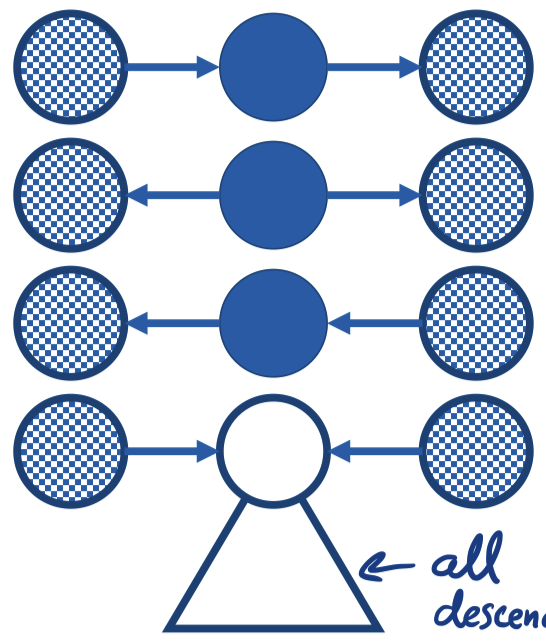
\includegraphics[width=0.3\columnwidth]{figures/d-sep.png}
    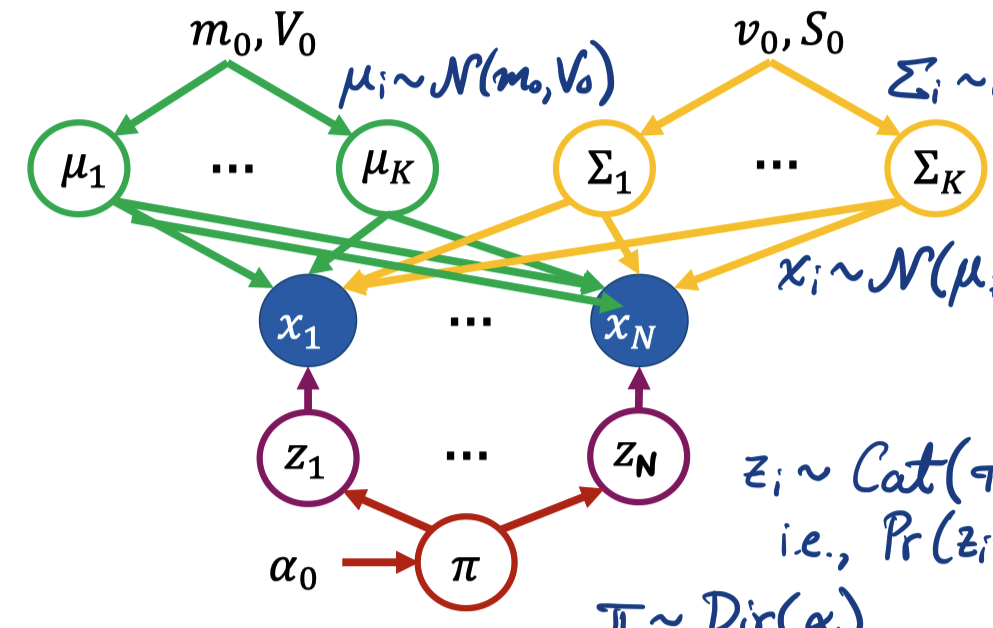
\includegraphics[width=0.50\columnwidth]{figures/GMM.png}
\end{center}
\vspace{-0.4cm}

\textbf{d-seperation}: for verifying conditional independence. Given with observed variable set $C$, if every path from variable $A$ to $B$ is blocked on probability graph, then $A$ and $B$ are independent condition on $C$. By this thm: (1) $z_i$, $z_j$ (2) $\mu$, $\pi$  (3) $\Sigma$, $\pi$ all independent condition on other parameter. Sampling procedure: \begin{scriptsize}
    (1) $z^{(t)} \leftarrow p\left(\cdot | x, \mu^{(t-1)}, \Sigma^{(t-1)}\right)$, (2) $\mu^{(t)} \leftarrow p\left(\cdot | x, \Sigma^{(t-1)}, z^{(t)}\right)$, (3) $\Sigma^{(t)} \leftarrow p\left(\cdot | x, \mu^{(t)}, z^{(t)}\right)$, (4) $\pi^{(t)} \leftarrow p\left(\cdot | x, z^{(t)}\right)$
\end{scriptsize}

\subsection*{BI for Non-Parametric GMM}
\textbf{Goal}: sample from infinite categorical distri.

\textbf{Dirichlet Process (DP)}: $\Theta$ parameter space, $H$ prior distri on $\Theta$, $A_1, \cdots, A_r$ arbitrary partition of $\Theta$. $G$ a categorical distribution over $\{A_i\}$ is  $G $\textasciitilde$ \mathrm{DP}(\alpha, H)$ if $\left(G\left(A_{1}\right), \ldots, G\left(A_{r}\right)\right) $\textasciitilde$ \operatorname{Dir}\left(\alpha H\left(A_{1}\right), \ldots, \alpha H\left(A_{r}\right)\right)$.

\textbf{Posterior}: $G | \{\theta_{i}\}_{i=1}^n $\textasciitilde$ \operatorname{DP}\left(\alpha+n, \frac{\alpha H + \sum_{i=1}^{n} \delta_{\theta_{i}}}{\alpha+n}\right)$

\textbf{Condition on $\theta$, Margin over $G$}: $\theta_{n+1} \mid \theta_{1}, \ldots, \theta_{n} $\textasciitilde$ \frac{1}{\alpha+n}\left(\alpha H+\sum_{i=1}^{n} \delta_{\theta_{i}}\right)$, Leads to CRP

\subsection*{Three Methods of Sampling from DP}

In $K\to\infty$ GMM, $\theta$ in DP is $z$, $G$ is $\pi$. 

\textbf{(1) Chinese Restaurant Process (CRP)}, sample $z$, marginalize over $\pi$: \\
$p(z_n = k| \theta_{i < n}) = 
\begin{cases}
    n_k / (\alpha + n - 1) \text{, existing }k \\
    \alpha / (\alpha + n - 1) \text{, new }k 
\end{cases}
$

\textbf{Expect \# of Class} $\sum_{i=1}^{n} \frac{\alpha}{\alpha+i-1} $\textasciitilde$eq \alpha \log \left(1+\frac{n}{\alpha}\right)$

\textbf{(2) Stick-breaking Construction} samples $\pi$: $\beta_{k} $\textasciitilde$ \operatorname{Beta}(1, \alpha)$, $\theta_{k}^{*} $\textasciitilde$ H$, $\pi_{k}=\beta_{k} \prod_{l=1}^{k-1}\left(1-\beta_{l}\right)$

\textbf{(3)} Marginalize over $\mu, \Sigma$ when sampling $z$ (if intractable), less variance (Rao-Blackwall).

\textbf{Exchangeability}: $p(\{\theta_i\}) = \prod_{n=1}^N p(\theta_n | \{\theta_{i<n}\})$ unchanged after permuting sampling order.

\textbf{DeFinetti’s Thm} any exchangeable distri is a mixture model $P\left(\{\theta_{i}\}\right)=\int \prod_{i=1}^{n} G\left(\theta_{i}\right) d P(G)$


    \section{PAC Learning}

Definitions:
\begin{itemize}
    \item A learning algorithm $\mathcal{A}$ can learn $c\in C$ if there is a poly(.,.), s.t. for (1) any distribution $\mathcal{D}$ on $\mathcal{X}$ and (2) $\forall 0<\epsilon<\frac{1}{2},0<\delta<\frac{1}{2}$, $\mathcal{A}$ outputs $\hat{c}\in \mathcal{H}$ given a sample of size at least poly($\frac{1}{\epsilon}$, $\frac{1}{\delta}$, size($c$)) such that $P(\mathcal{R}(\hat{c})-\inf_{c\in C}\mathcal{R}(c)\le\epsilon) \ge 1-\delta$.
    \item $\mathcal{A}$ is called an efficient PAC algorithm if it runs in polynomial of $\frac{1}{\epsilon}$ and $\frac{1}{\delta}$.
    \item $C$ is (efficiently) PAC-learnable from $\mathcal{H}$ if there is an algorithm $\mathcal{A}$ that (efficiently) learns $C$ from $\mathcal{H}$.
\end{itemize}

VC inequality:
\begin{itemize}
    \item For an ERM $\hat{c}^*_n$, $\mathbf{P}\left(\mathcal{R}\left(\hat{c}_{n}^{*}\right)-\inf _{c \in \mathcal{C}} \mathcal{R}(c)>\epsilon\right) \leq 2|\mathcal{C}| \exp \left(-\frac{n \epsilon^{2}}{2}\right)$.
    \item Finite VC-dimension means PAC-learnable.
\end{itemize}

    \section{Appendix}

$\frac{\partial}{\partial \Sigma} \log|\Sigma| = \Sigma^{-T}$.


\end{multicols*}
\end{document}
